% =============================================================================
%  ICEIR 2026 submission - SensitiveAI
%  Template: Springer LNNS (Lecture Notes in Networks and Systems), which uses
%  the LNCS "llncs" document class.  Compile with pdflatex + bibtex (splncs04).
%
%  NOTE TO AUTHORS: fill in the real author names, affiliations and ORCIDs
%  below (placeholders marked TODO), then compile:
%      pdflatex main
%      bibtex   main
%      pdflatex main
%      pdflatex main
% =============================================================================
\documentclass[runningheads]{llncs}

\usepackage[T1]{fontenc}
\usepackage[utf8]{inputenc}
\usepackage{graphicx}
\usepackage{booktabs}
\usepackage{multirow}
\usepackage{amsmath}
\usepackage{amssymb}
\usepackage{url}
\usepackage{tikz}
\usetikzlibrary{arrows.meta,positioning,fit,backgrounds,calc}
\usepackage[hidelinks]{hyperref}

% Pack floats more tightly so tables/figures share text pages instead of
% creating half-empty float pages (keeps the paper within the 12--15 page limit).
\renewcommand{\topfraction}{1.0}
\renewcommand{\bottomfraction}{1.0}
\renewcommand{\textfraction}{0.05}
\renewcommand{\floatpagefraction}{0.9}
\setcounter{totalnumber}{6}

% Tighten the whitespace between floats and the surrounding text so the many
% tables and figures share text pages without visibly large gaps.
\setlength{\textfloatsep}{4pt plus 2pt minus 2pt}
\setlength{\floatsep}{4pt plus 2pt minus 2pt}
\setlength{\intextsep}{4pt plus 2pt minus 2pt}
\setlength{\abovecaptionskip}{3pt}
\setlength{\belowcaptionskip}{1pt}

% Allow TeX to stretch lines slightly so long unbreakable tokens (model names,
% inline math) do not overflow the margin.
\setlength{\emergencystretch}{3em}

\newcommand{\model}[1]{\textsc{#1}}

\begin{document}

\title{SensitiveAI: An Ablation Study of Optimization Recipes
       for Vietnamese Hate Speech Detection}
\titlerunning{SensitiveAI: Ablation of Optimization Recipes for Vietnamese HSD}

\author{
Pham Kha Vy\inst{1} \and
Cao Hong Nga\inst{1}\textsuperscript{*}
}

\authorrunning{P. K. Vy and C. H. Nga}

\institute{
FPT University, Can Tho, Vietnam\\
\email{phamkhavycm2004@gmail.com}\\
\email{caohongnga@gmail.com}\\
\textsuperscript{*}is the correspondent author.
}


\maketitle

\begin{abstract}
Hate speech on Vietnamese social media is a pressing moderation problem, and
fine-tuned multilingual transformers such as mDeBERTa-v3 are now a common
approach.  Reported gains, however, usually bundle several independent design
decisions---head, learning-rate schedule, loss, class weighting, curriculum and
decision rule---into one number, so it is unclear which decision matters.  We
present \emph{SensitiveAI}, a controlled ablation of six systems sharing one fixed
split, label mapping, backbone (\texttt{microsoft/mdeberta-v3-base}) and seed,
differing only in the optimisation recipe, each scored once on the ViHSD test set
(three classes HATE / OFFENSIVE / CLEAN, 83\% CLEAN).  All six land in a narrow
0.654--0.664 macro-F1 and 0.863--0.878 accuracy band; no pairwise macro-F1
difference is significant under a paired bootstrap, and the only significant paired
comparisons are in accuracy, where the focal-only probe buys the highest minority
recall by giving up \textsc{clean} recall and so loses accuracy.  A
multi-view head with discriminative learning rates reaches the best macro-F1
(0.6638), a focal-only continuation of the baseline gives the best HATE F1 (0.609)
and macro ROC-AUC (0.893), and the highest accuracy (0.878) belongs to the system
with the \emph{lowest} macro-F1---the classic imbalanced-classification trap.  A
three-stage curriculum whose later stages never won validation selection, and a
validation-searched threshold rule, did not improve over simpler recipes.  We
report the full protocol, bootstrap confidence intervals,
a confusion-matrix and error analysis, and the negative results, so the comparison
can be reproduced rather than re-argued.
\keywords{hate speech detection \and Vietnamese NLP \and mDeBERTa \and
          class imbalance \and ablation study \and reproducibility.}
\end{abstract}

\section{Introduction}
\label{sec:intro}

Vietnam has one of the fastest-growing social-media user bases in Southeast Asia,
and the volume of Vietnamese text platforms must moderate keeps rising.  Flagging
hateful and offensive comments automatically is therefore a practical prerequisite
for healthier communities, yet Vietnamese remains low-resource and its social-media
style is hard (code-switching, ``teencode,'' informal spellings, evasive
substitutions, dropped diacritics).

The release of \emph{UIT-ViHSD} \cite{luu2021vihsd}, a human-annotated corpus of
roughly 33k Vietnamese comments labelled \textsc{clean}, \textsc{offensive} or
\textsc{hate}, made supervised transformer fine-tuning a realistic default and a
standard benchmark for monolingual encoders such as PhoBERT \cite{nguyen2020phobert}
and multilingual ones such as mBERT and XLM-R
\cite{conneau2020xlmr,nguyen2022smtce,hoang2023vihos}.  Multilingual DeBERTa-v3
variants have become popular because they combine a large multilingual pre-training
corpus with disentangled attention \cite{he2021deberta,he2023debertav3}.

In parallel, many \emph{optimisation} tricks are routinely applied to imbalanced
text classification: a richer classification head, discriminative (layer-wise)
learning rates, multi-stage fine-tuning, class-weighted or focal losses
\cite{lin2017focal}, curriculum learning \cite{bengio2009curriculum}, and per-class
decision thresholds \cite{saito2015precision}.  In the literature these are usually
bundled together and reported as a single end-to-end improvement, which leaves a
practical question unanswered: \emph{which of these decisions actually moves the
number on Vietnamese hate speech detection, and by how much?}

This paper answers that with a \emph{controlled ablation}: six systems sharing one
backbone (\texttt{microsoft/mdeberta-v3-base}), one fingerprinted split, one frozen
label mapping, one tokenizer configuration and one seed, differing \emph{only} in
the optimisation recipe and each scored once on the held-out test set.  The chain
(Sect.~\ref{sec:method}) runs from a plain baseline, to a multi-view pooling head,
to a variant adding discriminative rates and class-weighted two-stage training, to a
three-stage curriculum.

Our contributions are:

\begin{itemize}
  \item A comparison of six optimisation recipes for three-class Vietnamese hate
        speech detection under one fixed split and seed, reported with split
        fingerprints, per-class metrics, bootstrap intervals and paired significance
        tests so it can be reproduced rather than re-argued.
  \item A multi-view classification head (first-token, masked-mean and masked-max
        pooling) attaining the best macro-F1 at essentially the same parameter
        count as the standard head.
  \item An empirical demonstration that the recipes are not uniformly better: no
        pairwise macro-F1 difference is significant (a failure to detect, not
        proof of equivalence), the most accurate system has one of the lowest
        macro-F1 scores, a three-stage curriculum never wins validation
        selection, and a validation-searched threshold collapses to the trivial
        $0.5$---negative results we discuss for applied moderation.
\end{itemize}

\section{Related Work}
\label{sec:related}

\subsection{Vietnamese Hate Speech Detection}
Hate speech detection is well studied for high-resource languages, but Vietnamese
resources appeared comparatively late.  The \emph{UIT-ViHSD} corpus
\cite{luu2021vihsd} is the reference three-class dataset for Vietnamese social
media; the VLSP 2019 shared task \cite{vu2020hsdvlsp} was an earlier benchmark, and
related resources include UIT-ViCTSD \cite{nguyen2021victsd} and ViHOS for
hate/offensive span detection \cite{hoang2023vihos}; the SMTCE benchmark
\cite{nguyen2022smtce} supplies the published numbers we reuse.  Vietnamese-specific
encoders have since raised the state of the art: ViDeBERTa \cite{tran2023videberta}
is a monolingual DeBERTa pre-trained on Vietnamese, ViSoBERT
\cite{nguyen2023visobert} adapts to social-media text and is, to our knowledge, the
strongest reported ViHSD encoder, ViHateT5 \cite{nguyen2024vihatet5} reformulates
the task as text-to-text, and pipelines such as PhoBERT-CNN
\cite{tran2022phobertcnn} report higher scores with steps outside our controlled
setting.

\subsection{Pre-trained Encoders}
Fine-tuning pre-trained transformers is the dominant approach, with PhoBERT
\cite{nguyen2020phobert} for Vietnamese and mBERT \cite{devlin2019bert} and XLM-R
\cite{conneau2020xlmr} for multilingual settings.  DeBERTa \cite{he2021deberta}
introduced disentangled attention and DeBERTaV3 \cite{he2023debertav3} replaced
masked-language modelling with replaced-token detection; the multilingual
checkpoint \texttt{microsoft/mdeberta-v3-base}, extending this to 100+ languages,
is the backbone used here.

\subsection{Learning under Class Imbalance}
ViHSD is strongly imbalanced and the minority classes are the main error source.
Common remedies re-weight the loss by training frequency---the effective number of
samples \cite{cui2019classbalanced} or the inverse frequency---use focal loss,
which down-weights easy examples \cite{lin2017focal}, or move the decision threshold
away from $0.5$.  Curriculum learning \cite{bengio2009curriculum} schedules
difficulty or label focus over time, and discriminative fine-tuning with layer-wise
rates was popularised by ULMFiT \cite{howard2018ulmfit}.  We fix the encoder and
optimiser family and vary exactly these factors; most prior ViHSD work reports a
single aggregate improvement, so we deliberately surface the negative findings that
single-number reports hide.

\section{Dataset}
\label{sec:dataset}

\subsection{UIT-ViHSD}
We use \emph{UIT-ViHSD} \cite{luu2021vihsd}, a human-annotated corpus of Vietnamese
social-media comments, each carrying exactly one label: \textsc{clean},
\textsc{offensive} (insulting but not hate speech) or \textsc{hate} (targeting a
person or protected group).

We follow the official train/dev/test partition.  Preprocessing is deliberately
light and label-preserving: strip leading/trailing whitespace, collapse runs of
whitespace, drop control characters, and drop only rows with no usable text (2
rows in train).  We \emph{keep} duplicates and do not lowercase, strip diacritics,
normalise teencode or truncate emoji, because those surface cues are part of the
signal.  This yields 33{,}398 comments (24{,}046 / 2{,}672 / 6{,}680 for
train/dev/test); the corpus has 33{,}400 rows---the difference is exactly the 2
empty-text train rows (Table~\ref{tab:splits}).  Comments are short and uneven
(test mean 47.5 characters, median 33; \textsc{hate} about twice as long as the
others).  The annotation study reports only moderate inter-annotator agreement
($\kappa\approx0.5$), which sets a ceiling on accuracy: some test comments are
genuinely ambiguous between \textsc{offensive} and \textsc{hate}, and no recipe
removes that label noise.

\subsection{Label Mapping and Imbalance}
\label{sec:imbalance}
The native ViHSD identifiers are (0 = \textsc{clean}, 1 = \textsc{offensive},
2 = \textsc{hate}); because the minority classes are the object of study, we freeze
a canonical mapping with the rare class first ($\textsc{hate}=0$,
$\textsc{offensive}=1$, $\textsc{clean}=2$), applied once and never changed.

The distribution is skewed and stable across splits: \textsc{clean} is 82--83\% of
every split, \textsc{hate} about 10\%, and \textsc{offensive} the smallest class at
6.6--7.9\% (test: 688 \textsc{hate}, 444 \textsc{offensive}, 5{,}548
\textsc{clean}).  Two consequences follow.  First, accuracy is misleading---a
degenerate \textsc{clean}-always classifier would score about $0.83$ yet be
useless---so macro-F1 is primary.  Second, offensive and hate speech share most
surface markers, so the interesting comparison is the trade-off between
minority-class F1 and the easy \textsc{clean} class.

\subsection{Fixed Split and Reproducibility}
The split must be identical for every system, so we store it as CSV files and record
each file's SHA-256 digest in a manifest copied into every run directory; all six
systems read the same three files and label mapping, leaving the recipe as the only
varying factor, with the test split scored once per system after hyper-parameters
are frozen on validation (Table~\ref{tab:splits}).

% Fixed split used by every system; digests are the first 12 hex digits of the
% full SHA-256 recorded in data/splits/split_manifest.json.
\begin{table}[t]
\centering
\small
\setlength{\tabcolsep}{4pt}
\caption{The fixed split stored once and reread by every system.  Counts are
comments after cleaning (Sect.~\ref{sec:dataset}).  The SHA-256 digest (first
12 hex digits of the full value in the released manifest) is copied into each run
directory and re-checked before training.}
\label{tab:splits}
\begin{tabular}{lrrrrl}
\toprule
Split & Comments & HATE & OFF. & CLEAN & SHA-256 \\
\midrule
train      & 24{,}046 & 2{,}556 & 1{,}605 & 19{,}885 & \texttt{f705ffe94d41} \\
validation & 2{,}672  & 270     & 212     & 2{,}190  & \texttt{6aa552aafb92} \\
test       & 6{,}680  & 688     & 444     & 5{,}548  & \texttt{d8f9ae7ddd8c} \\
\bottomrule
\end{tabular}
\end{table}


\subsection{Duplication Across Splits}
Because we keep duplicates, we measured their cross-split prevalence.  The official
ViHSD partition reuses comments: after case-folding, $895$ of the $6{,}680$ test
comments ($13.4\%$) have an exact duplicate in train or validation and $118$
duplicated strings carry conflicting labels, a property of the public split that
can only flatter absolute scores.  Table~\ref{tab:duplicate-free} re-scores all six
systems on the $5{,}785$ duplicate-free comments: accuracy drops by $0.3$--$0.5$
points for every system while macro-F1 and its ordering barely move (M3 still
highest at $0.6654$; only the two lowest systems swap, by $0.0003$), so the
conclusions do not rest on the overlap (Sect.~\ref{sec:threats}).

% AUTO-GENERATED by scripts/08_check_leakage.py - do not edit by hand.
\begin{table}[h]
\centering
\footnotesize
\setlength{\tabcolsep}{4pt}
\caption{Full vs.\ the 5,785 duplicate-free test comments (Sect.~\ref{sec:dataset}).  Accuracy drops for every system while macro-F1 and its ordering are essentially unchanged, so the conclusions do not rest on the overlap (Sect.~\ref{sec:threats}).}
\label{tab:duplicate-free}
\begin{tabular}{lcccc}
\toprule
 & \multicolumn{2}{c}{Accuracy} & \multicolumn{2}{c}{Macro-F1} \\
\cmidrule(lr){2-3} \cmidrule(lr){4-5}
System & Full & Dup-free & Full & Dup-free \\
\midrule
M1 & 0.8734 & 0.8681 & 0.6545 & 0.6533 \\
M2 & 0.8762 & 0.8719 & 0.6575 & 0.6576 \\
M3 & 0.8754 & 0.8721 & \textbf{0.6638} & \textbf{0.6654} \\
M4 & 0.8731 & 0.8698 & 0.6590 & 0.6601 \\
M5 & \textbf{0.8783} & \textbf{0.8748} & 0.6536 & 0.6537 \\
M6 & 0.8633 & 0.8588 & 0.6604 & 0.6606 \\
\bottomrule
\end{tabular}
\end{table}


\section{Methodology}
\label{sec:method}

\subsection{Backbone and Common Configuration}
All six systems use the same encoder, \texttt{microsoft/mdeberta-v3-base}
\cite{he2023debertav3,liu2024mdeberta}, a multilingual DeBERTa-v3 model with a
hidden size of 768 and 12 transformer layers.  The encoder is left untouched;
the systems differ only in what sits on top of it and in how it is trained.

The training configuration is fixed across systems (Sect.~\ref{sec:setup}).
The seed is 42 and all runs shared device and library versions; the tokenizer,
label mapping and split are identical everywhere (bitwise determinism across
hardware is not claimed).  Figure~\ref{fig:architecture} overviews the pipeline and
the points at which the six systems differ.

\begin{figure}[t]
\centering
\resizebox{0.55\textwidth}{!}{%
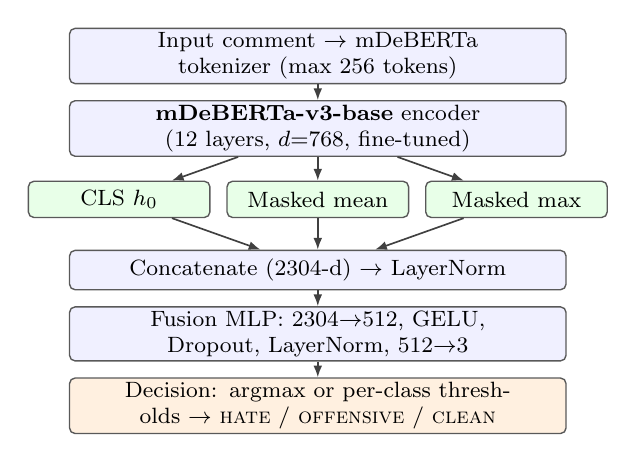
\begin{tikzpicture}[
  font=\footnotesize,
  >=Latex,
  node distance=2mm,
  box/.style={rectangle, rounded corners=2pt, draw=black!65, line width=0.5pt,
              fill=blue!6, align=center, text width=62mm, minimum height=5mm, inner sep=1.5pt},
  view/.style={rectangle, rounded corners=2pt, draw=black!65, line width=0.5pt,
              fill=green!9, align=center, text width=22mm, minimum height=4.6mm, inner sep=1.5pt},
  outbox/.style={rectangle, rounded corners=2pt, draw=black!65, line width=0.5pt,
              fill=orange!12, align=center, text width=62mm, minimum height=5mm, inner sep=1.5pt},
  ar/.style={-{Latex[length=1.5mm]}, line width=0.6pt, draw=black!75}
]
\node[box] (input) {Input comment $\rightarrow$ mDeBERTa tokenizer (max 256 tokens)};
\node[box, below=of input] (enc) {\textbf{mDeBERTa-v3-base} encoder (12 layers, $d{=}768$, fine-tuned)};
\node[view, below=3mm of enc] (mean) {Masked mean};
\node[view, left=2mm of mean] (cls) {CLS $h_0$};
\node[view, right=2mm of mean] (max) {Masked max};
\node[box, below=4mm of mean] (concat) {Concatenate (2304-d) $\rightarrow$ LayerNorm};
\node[box, below=of concat] (mlp) {Fusion MLP: $2304{\to}512$, GELU, Dropout, LayerNorm, $512{\to}3$};
\node[outbox, below=of mlp] (out) {Decision: argmax or per-class thresholds $\rightarrow$
   \textsc{hate} / \textsc{offensive} / \textsc{clean}};

\draw[ar] (input) -- (enc);
\draw[ar] (enc) -- (cls);
\draw[ar] (enc) -- (mean);
\draw[ar] (enc) -- (max);
\draw[ar] (cls) -- (concat);
\draw[ar] (mean) -- (concat);
\draw[ar] (max) -- (concat);
\draw[ar] (concat) -- (mlp);
\draw[ar] (mlp) -- (out);
\end{tikzpicture}}
\caption{The SensitiveAI pipeline.  All six systems share the encoder and the
decision stage; M2--M5 add the multi-view pooling head shown here, whereas M1 and
M6 keep the standard first-token head.  The recipes ablated on top are the
baseline, the multi-view head plus DLR and two-stage training (weighted CE then
focal), and the three-stage concept curriculum.}
\label{fig:architecture}
\end{figure}

\subsection{Systems and the Ablation Chain}
\label{sec:chain}
The systems form a chain in which each step swaps a whole recipe of decisions
(head, losses, learning rates, stages and decision rule together), plus two probes
that target a single component.  We label them \textbf{M1}--\textbf{M6} and use
these labels throughout:

\begin{enumerate}
  \item \textbf{M1}, \model{sensitiveai-vi} (baseline): standard Hugging Face
        head, single rate $3\times10^{-5}$, unweighted cross-entropy, argmax.
  \item \textbf{M2}, \model{sensitiveai-vi-custom}: baseline plus the multi-view
        head (Sect.~\ref{sec:head}).
  \item \textbf{M3}, \model{sensitiveai-vi-customdlr2stage}: custom head plus
        discriminative learning rates, two-stage training, class-weighted
        cross-entropy then focal loss, and searched thresholds
        (Sect.~\ref{sec:dlr}).
  \item \textbf{M4}, \model{sensitiveai-vi-custom-curriculum}: custom head plus a
        three-stage ``concept'' curriculum instead of the two stages
        (Sect.~\ref{sec:curriculum}).
  \item \textbf{M5}, \model{sensitiveai-vi-customdlr2stage-ext}: probe continuing
        M3's stage~1 for 15 further epochs, to test whether that optimum was a
        peak or merely the end of the schedule.
  \item \textbf{M6}, \model{sensitiveai-vi-stage2}: probe applying \emph{only}
        the stage-2 recipe (focal loss, class weights, lower rate) on the
        baseline checkpoint, keeping the standard head.
\end{enumerate}

\subsection{Multi-View Classification Head}
\label{sec:head}
The standard DeBERTa head places a pooler on the first token and a single linear
layer on top, $\mathbf{h}[0] \rightarrow \mathrm{Linear}(768{\to}768)+\tanh
\rightarrow \mathrm{Linear}(768{\to}3)$, so the decision rests on one
token---fragile for short, noisy comments where a trigger word, not the first
token, decides the label.  The custom head keeps the encoder and changes only what
follows.  With final states $\mathbf{H}\in\mathbb{R}^{L\times 768}$ and mask
$\mathbf{m}\in\{0,1\}^{L}$, the three views are
$\mathbf{z}_{\mathrm{cls}}=\mathbf{H}[0]$,
$\mathbf{z}_{\mathrm{mean}}=\tfrac{\sum_{l} m_l\,\mathbf{H}[l]}{\sum_l m_l}$ and
$\mathbf{z}_{\mathrm{max}}=\max_{l:\,m_l=1}\mathbf{H}[l]$, where the masked mean
ignores padding and the masked max maximises over valid positions only.  The views
are concatenated into a 2304-dimensional vector, LayerNorm-normalised, and passed
through a fusion block $\mathrm{Linear}(2304{\to}512)\rightarrow
\mathrm{GELU}\rightarrow \mathrm{Dropout}(0.1)\rightarrow \mathrm{LayerNorm}
\rightarrow \mathrm{Dropout}(0.1)\rightarrow \mathrm{Linear}(512{\to}3)$; the
512-unit bottleneck adds a non-linear, regularised boundary.  Since the encoder,
data and optimiser are unchanged, M1 vs.\ M2 is the one clean single-factor step in
the chain and isolates the head.

\subsection{Losses and Class Weighting}
\label{sec:losses}
The baseline uses unweighted cross-entropy; later systems use \emph{weighted
cross-entropy} (class weights = inverse square root of the training frequency,
normalised to mean one), \emph{focal loss} \cite{lin2017focal} with $\gamma=2$ and
$\alpha_{\textsc{hate}}=0.5$,
$\alpha_{\textsc{offensive}}=\alpha_{\textsc{clean}}=0.25$ combined with those
weights, or \emph{manual weights} $\textsc{hate}{:}3,\ \textsc{offensive}{:}2,\
\textsc{clean}{:}1$ for the curriculum's final stage.  Class weights are computed
on the training split only.

\subsection{Discriminative Learning Rates and Two-Stage Training}
\label{sec:dlr}

Two optimisation ideas are combined in M3.

\paragraph{Discriminative (layer-wise) learning rates.}
Following ULMFiT \cite{howard2018ulmfit}, parameters are split into four groups
with decreasing rates from head to input (embeddings $5\times10^{-6}$, lower half
$1\times10^{-5}$, upper half $2\times10^{-5}$, head $1\times10^{-4}$), so the
task-specific head adapts quickly from random initialisation while pre-trained
representations avoid catastrophic forgetting.  The encoder starts from the same
checkpoint as M1 and M2, so the recipes share one initialisation.

\paragraph{Two-stage training.}
Training has two stages of up to 15 epochs each: \emph{stage~1} stabilises the
representation under class-weighted cross-entropy at rate $2\times10^{-5}$ with
warmup $0.1$; \emph{stage~2} continues from its checkpoint with lower rates and
focal loss, which down-weights easy examples.  Here the selected
checkpoint was the \emph{end of stage~1} (validation macro-F1 $0.7089$); focal
stage~2 never improved on it and stopped early, so M3's headline number comes from
discriminative rates plus class-weighted cross-entropy, not focal loss.

\paragraph{Label-specific decision thresholds.}
The decision rule is changed from argmax to per-class thresholds: a label is
accepted when its probability reaches its own threshold, the highest-probability
accepted label wins, and if none passes the plain argmax is used.  The thresholds
are searched to maximise validation macro-F1 by coordinate ascent over a
101-point grid in $[0,1]$ from $0.5$, on the validation split only, then frozen
and applied unchanged to the test pass.

\subsection{Three-Stage Curriculum Concept Training}
\label{sec:curriculum}

M4 replaces the two stages with a three-stage curriculum
\cite{bengio2009curriculum} that shapes the representation with easier binary
sub-problems before the final decision: \emph{stage~1} targets
``\textsc{offensive} versus anything else'', \emph{stage~2} ``\textsc{hate} versus
anything else'', and \emph{stage~3} returns to the three-class objective with
class weights $\textsc{hate}{:}3,\ \textsc{offensive}{:}2,\ \textsc{clean}{:}1$.
The full dataset is used in \emph{every} stage (a concept's negative class is the
other two classes) and the three-way head is kept throughout, the concept loss
simply re-reading the three logits as a binary objective.  Each stage runs up to 10
epochs with rates decreasing from $2\times10^{-5}$ to $1\times10^{-5}$
(stage~3 raises this slightly to $1.5\times10^{-5}$) and the discriminative
grouping of Sect.~\ref{sec:dlr}.  M4
asks whether a finer sequence of increasingly difficult stages beats M3's two.
All three stages run, but no epoch after the first improves the validation
macro-F1 used for checkpoint selection (best $0.694$), so the finer sequence does
not win.

\section{Experimental Setup}
\label{sec:setup}

\subsection{Hardware and Software}
All experiments were run on a single workstation with an NVIDIA GeForce RTX
4060 Laptop GPU (8\,GB), CUDA 12.6, PyTorch 2.13 and Python 3.11, using the
Hugging Face Transformers library \cite{wolf2020transformers}.  The
\texttt{mdeberta-v3-base} encoder has $278.2$M parameters.  The standard Hugging
Face head (a 768-d pooler plus a 3-way linear layer) adds $0.59$M, so the
standard-head systems (M1, M6) total $278.8$M; the multi-view head adds
$1.19$M, so the custom-head systems (M2--M5) total $279.4$M.  The largest gap
between any two systems is thus $+0.21\%$ of the parameters, and we treat them as
of essentially identical size.

\subsection{Training Protocol}
All systems share one configuration: AdamW \cite{loshchilov2019adamw} with weight
decay 0.01, a linear schedule with warmup $0.05$--$0.1$, batch size 16 with
gradient accumulation~2 (effective 32), gradient clipping at norm 1.0, sequence
length 256 tokens, bf16 training (fp32 for the latency benchmark), and up to
15--30 epochs depending on the recipe.  Early stopping monitors validation
macro-F1 with patience 6 and restores the best checkpoint.  The systems differ
only in the encoder initialisation, the number of stages, the loss sequence and
the class-weighting scheme (Sect.~\ref{sec:chain}); the test split is evaluated
exactly once per system with the checkpoint selected on validation.
Table~\ref{tab:training-details} lists the resolved configuration and the frozen
checkpoint (best epoch and its validation macro-F1) for each system.  Every system
reads the same three split files (verified by SHA-256 digest) and label mapping,
and all class weights and thresholds are estimated on training and validation only,
never on test; only the head, learning rates, number of stages and loss vary.

% AUTO-GENERATED by scripts/06_analyze_significance.py - do not edit by hand.
\begin{table}[t]
\centering
\small
\setlength{\tabcolsep}{4pt}
\caption{Training configuration and the validation checkpoint that was frozen for the test pass (M1--M6, Sect.~\ref{sec:chain}). AdamW, linear schedule, effective batch size 32 and sequence length 256 are shared by all systems. ``init`` is the encoder the first stage starts from; ``best ep.`` is the epoch whose validation macro-F1 was highest (it can lie in an earlier stage).}
\label{tab:training-details}
\begin{tabular}{lcccccc}
\toprule
System & init & stages & loss & class w. & best ep. & val M-F1 \\
\midrule
M1 & pre-trained & 1 & CE & none & 9 & 0.6961 \\
M2 & pre-trained & 1 & CE & none & 14 & 0.6957 \\
M3 & chained & 2 & CE $\to$ focal & inv-sqrt & 15\,(s1) & 0.7089 \\
M4 & M3 best & 3 & concept $\to$ CE & manual & 1\,(s1) & 0.6942 \\
M5 & M3 stage-1 & 1 & CE & inv-sqrt & 3 & 0.7072 \\
M6 & M1 best & 1 & focal & inv-sqrt & 4 & 0.6928 \\
\bottomrule
\end{tabular}
\end{table}


\subsection{Metrics}
Because of the imbalance described in Sect.~\ref{sec:imbalance}, we treat
\emph{macro-averaged F1} as primary and report accuracy only as a diagnostic,
alongside per-class precision, recall and F1 and macro ROC-AUC / average precision
(AP), since precision-recall summaries are more trustworthy than ROC under
imbalance \cite{saito2015precision}.  Calibration uses the top-label expected
calibration error (ECE, 10 bins); significance uses a percentile bootstrap
(macro-F1) and the exact McNemar test (accuracy).

\section{Results}
\label{sec:results}

\subsection{Headline Comparison}
Table~\ref{tab:model-comparison} reports the test results.  The systems are
tightly clustered---macro-F1 spans $0.6536$--$0.6638$ ($1.0$ pt) and accuracy
$0.8633$--$0.8783$---and these spreads sit inside sampling noise: the 95\% bootstrap
intervals on macro-F1 are about $\pm0.019$ wide (Table~\ref{tab:confidence}), so
every pairwise gap lies within a single interval and none is significant
(Sect.~\ref{sec:significance}).  The observations below are directions of effect,
not established rankings.

% AUTO-GENERATED by src/comparison/compare_models.py - do not edit by hand.
\begin{table}[t]
\centering
\small
\setlength{\tabcolsep}{4pt}
\caption{Comparison of the six systems (M1--M6, Sect.~\ref{sec:chain}) on the ViHSD test set under one fixed split; M-F1/W-F1: macro/weighted F1; HATE/OFF./CLEAN: per-class F1; AUC/AP: macro ROC-AUC / average precision.}
\label{tab:model-comparison}
\begin{tabular}{lcccccccc}
\toprule
Model & Acc. & M-F1 & W-F1 & HATE & OFF. & CLEAN & AUC & AP \\
\midrule
M1 & 0.8734 & 0.6545 & 0.8705 & 0.5864 & 0.4367 & 0.9405 & 0.8873 & \textbf{0.6599} \\
M2 & 0.8762 & 0.6575 & 0.8709 & 0.5830 & 0.4493 & 0.9403 & 0.8842 & 0.6484 \\
M3 & 0.8754 & \textbf{0.6638} & \textbf{0.8730} & 0.5943 & \textbf{0.4561} & 0.9409 & 0.8594 & 0.6254 \\
M4 & 0.8731 & 0.6590 & 0.8701 & 0.5847 & 0.4535 & 0.9389 & 0.8500 & 0.6367 \\
M5 & \textbf{0.8783} & 0.6536 & 0.8711 & 0.5843 & 0.4350 & \textbf{0.9415} & 0.8096 & 0.6124 \\
M6 & 0.8633 & 0.6604 & 0.8679 & \textbf{0.6088} & 0.4382 & 0.9344 & \textbf{0.8930} & 0.6534 \\
\bottomrule
\end{tabular}
\end{table}


The full recipe (M3) is best by macro-F1 ($\mathbf{0.6638}$) and OFFENSIVE F1
($0.4561$); the extended probe (M5) has the highest accuracy ($\mathbf{0.8783}$)
and CLEAN F1 yet the lowest macro ROC-AUC ($0.8096$); the stage-2 probe (M6) has
the highest HATE F1 ($\mathbf{0.6088}$), ROC-AUC ($\mathbf{0.8930}$) and AP, but
the lowest accuracy; and the custom head alone moves macro-F1 only to $0.6575$.

\subsection{Ablation Reading}
Table~\ref{tab:model-comparison} gives the chain: each step swaps a \emph{whole}
recipe, so a gap is the combined effect of its changes, not a single-factor
estimate.  The custom head adds $+0.30$ macro-F1 (M1$\to$M2); discriminative rates,
two-stage class-weighted training and a threshold search another $+0.63$
(M2$\to$M3); and the curriculum gives back $0.48$ (M3$\to$M4).  The two probes are
most informative: class-weighted focal loss on a \emph{standard} head (M6) reaches
$0.6604$, beating the baseline, the custom head and the curriculum at the best HATE
F1 and ranking quality; extending stage~1 (M5) \emph{hurts} (macro-F1 $0.6536$,
ROC-AUC $0.8096$), evidence that further cross-entropy training drifts to the
majority class.  M3's selected checkpoint was the end of its cross-entropy stage
(val. macro-F1 $0.7089$ at epoch~15), so its focal stage never helped: the same
ingredient succeeds or fails depending on what precedes it.

\subsection{Accuracy Versus Macro-F1}
\label{sec:trap}
The clearest lesson is the accuracy/macro-F1 contrast: the most accurate system
(M5, $0.8783$) is the one \emph{not} to deploy---it has the worst OFFENSIVE
recall ($0.381$) and the weakest ranking quality, because majority-class
prediction is rewarded by accuracy and punished by macro-F1.  Accuracy-based
selection is therefore inadvisable here, consistent with the classical preference
for precision-recall over ROC under imbalance \cite{saito2015precision}.

\subsection{Training Dynamics}
Validation accuracy plateaus within about five epochs in a narrow $0.86$--$0.88$
band, but the selected checkpoints fall at different epochs (9 for M1, 15 for M3,
3 for M5) and validation loss turns upward while training loss keeps falling, so
early stopping on validation macro-F1---not loss---selects the checkpoint.

\subsection{Per-Class Behaviour and Error Analysis}
The per-class breakdown (Table~\ref{tab:model-comparison}) localises the
difficulty: CLEAN is nearly solved (F1 $0.93$--$0.94$) while OFFENSIVE stays at
$0.43$--$0.46$ and HATE at $0.58$--$0.61$ for every system.  The full recipe
rebalances the minority classes---HATE recall $0.538\to0.573$ and OFFENSIVE
precision $0.434\to0.474$ at unchanged recall---while the curriculum and the
focal-only probe buy HATE recall up to $0.647$ (M6) by cutting CLEAN recall to
$0.922$.

\begin{figure}[t]
\centering
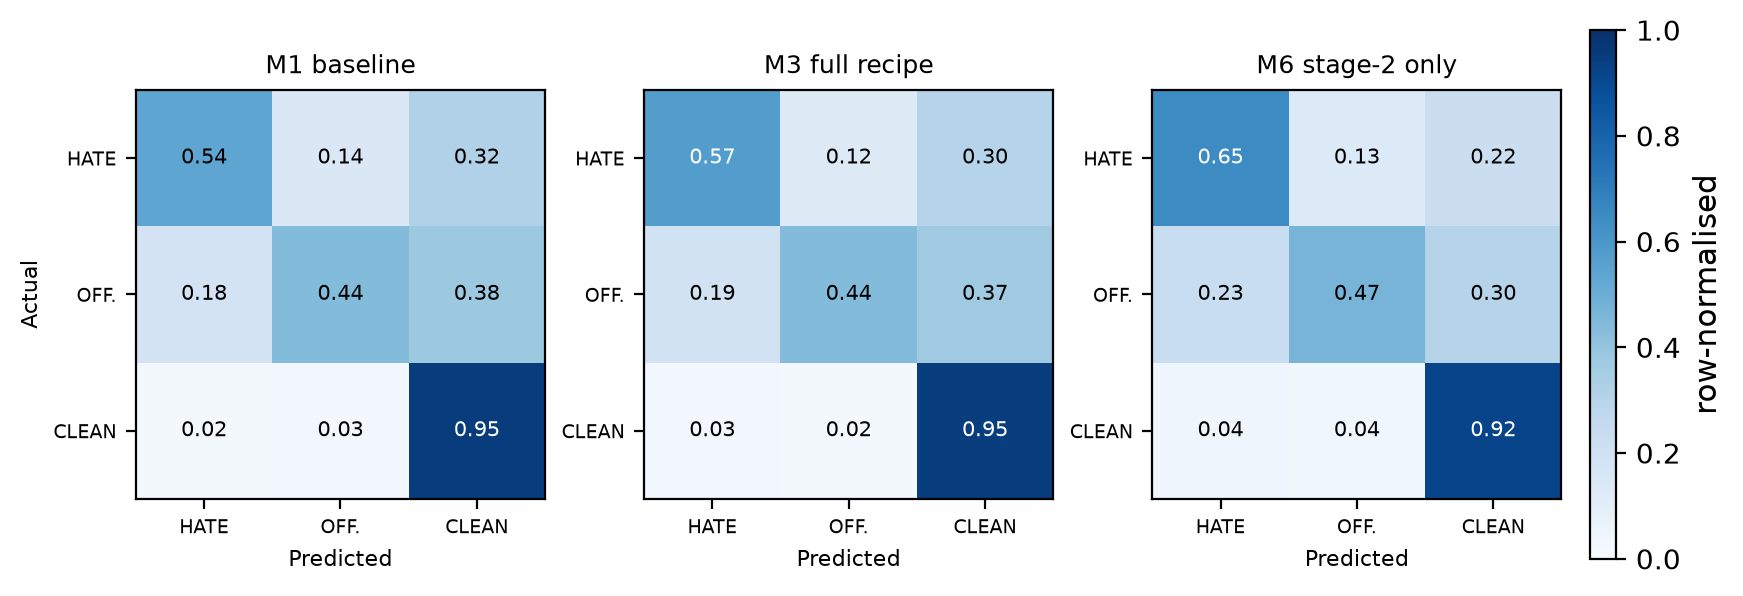
\includegraphics[width=0.62\textwidth]{figures/confusion_matrices.png}
\caption{Row-normalised test confusion matrices for the baseline (M1), the best
macro-F1 system (M3) and the focal-only probe (M6).  Every system shares one
failure mode: \textsc{offensive} comments sent to \textsc{hate} or
\textsc{clean}, and \textsc{hate} diluted into its neighbours; the systems differ
by a few percent along these rows, not by a change of failure mode.}
\label{fig:confusion}
\end{figure}

Figure~\ref{fig:confusion} confirms the shared failure mode: the
\textsc{offensive} row is weakest ($38$--$46\%$ misrouted) and \textsc{hate} is
diluted into its neighbours, while \textsc{clean} is almost never touched.
Splitting the test set by surface cues (M3) shows the difficulty is lexical
rather than syntactic: it is worst on \emph{very long} comments (accuracy $0.786$;
OFFENSIVE recall $0.14$) and on those \emph{without diacritics} or with
\emph{teencode}, and best on short comments---exactly the long, teencode-heavy
minority comments a majority shortcut discards.

\subsection{Statistical Significance and Calibration}
\label{sec:significance}
Because the spread is so small we re-analyse the frozen predictions with a
percentile bootstrap ($10{,}000$ resamples, seed 42) for macro-F1 and the exact
two-sided McNemar test for correctness; the two tests answer different questions
and are reported separately.  Table~\ref{tab:confidence} gives the intervals, the
top-label expected calibration error (ECE) and the paired comparisons.

% AUTO-GENERATED by scripts/06_analyze_significance.py - do not edit by hand.
\begin{table}[t]
\centering
\footnotesize
\setlength{\tabcolsep}{2pt}
\caption{Post-hoc statistics on the frozen test predictions. \emph{Top:} accuracy and macro-F1 with 95\% percentile bootstrap intervals (10,000 resamples of the 6,680 test items) and the top-label expected calibration error (ECE, 10 bins). \emph{Bottom:} paired comparisons, $A$ minus $B$, with a 95\% paired-bootstrap interval on macro-F1; $p_{\text{F1}}$ is the paired-bootstrap $p$-value and $p_{\text{acc}}$ the exact two-sided McNemar $p$-value on the two systems' correctness. $^{\dagger}$ marks $p<0.05$ after a Holm--Bonferroni correction over the seven comparisons below; values below $0.001$ are shown as $<0.001$. No macro-F1 gap is significant; the only differences that survive correction are the two accuracy gaps involving M6, discussed in the text.}
\label{tab:significance}
\label{tab:confidence}
\begin{tabular}{lcccc}
\toprule
System & Acc. [95\% CI] & M-F1 [95\% CI] & ECE & \\
\midrule
M1 & 0.8734 [0.8653, 0.8813] & 0.6545 [0.6353, 0.6736] & 0.106 & \\
M2 & 0.8762 [0.8681, 0.8841] & 0.6575 [0.6375, 0.6771] & 0.111 & \\
M3 & 0.8754 [0.8672, 0.8835] & 0.6638 [0.6442, 0.6823] & 0.120 & \\
M4 & 0.8731 [0.8648, 0.8810] & 0.6590 [0.6396, 0.6779] & 0.119 & \\
M5 & 0.8783 [0.8702, 0.8861] & 0.6536 [0.6334, 0.6728] & 0.118 & \\
M6 & 0.8633 [0.8549, 0.8716] & 0.6604 [0.6424, 0.6781] & 0.068 & \\
\midrule
$A-B$ & $\Delta$M-F1 [95\% CI] & $p_{\text{F1}}$ & $\Delta$Acc & $p_{\text{acc}}$ \\
\midrule
M3 $-$ M1 & +0.0092 [-0.0082, +0.0269] & 0.298 & +0.0021 & 0.526 \\
M3 $-$ M2 & +0.0062 [-0.0060, +0.0186] & 0.328 & -0.0007 & 0.788 \\
M3 $-$ M4 & +0.0047 [-0.0051, +0.0144] & 0.342 & +0.0024 & 0.217 \\
M3 $-$ M6 & +0.0033 [-0.0124, +0.0188] & 0.678 & +0.0121 & $<0.001$$^{\dagger}$ \\
M3 $-$ M5 & +0.0101 [-0.0023, +0.0228] & 0.113 & -0.0028 & 0.217 \\
M5 $-$ M1 & -0.0009 [-0.0185, +0.0164] & 0.906 & +0.0049 & 0.110 \\
M6 $-$ M1 & +0.0059 [-0.0071, +0.0191] & 0.377 & -0.0100 & $<0.001$$^{\dagger}$ \\
\bottomrule
\end{tabular}
\end{table}


Two conclusions follow.  First, \textbf{no pairwise macro-F1 difference is
significant}: the largest gap (M3$-$M5, $+0.010$) has paired interval
$[-0.002,+0.023]$ containing zero ($p=0.11$).  Second, \textbf{the accuracy ranking
is more stable, and there the McNemar test does reject}: M6 is significantly
\emph{less} accurate than both M3 and M1 ($p<0.001$ each), because it trades
minority recall for majority predictions---the one paired difference in the whole
study that survives correction.  Calibration also differs (focal-only probe best,
ECE $0.068$; full recipe worst, $0.120$), so the defensible claim is not ``M3 is
best'' but ``the recipes tie on macro-F1, and the choice should rest on secondary
criteria (minority recall, calibration, cost)''.

\subsection{Ranking Quality and Decision Rules}
Ranking tells a different story from thresholded F1: macro ROC-AUC peaks for M6
($0.8930$) and M1 ($0.8873$) while M3 sits at $0.8594$, consistent with their
differing calibration.  Only M3--M6 searched per-class thresholds, and only M4
found non-trivial values ($0.01/0.5/0.64$, validation macro-F1 $0.694\to0.697$)---a
gain that did not transfer to test; elsewhere the search returned the trivial
$0.5$, so a searched rule adds nothing over calibrated argmax here.

\subsection{Inference Cost}
Latency (fp32, same GPU/tokenizer/length/batch, indicative only) clusters at
$11.0$--$11.6$\,ms/sample for the custom-head systems, but the standard-head
baseline (M1) measured $28.1$\,ms against $10.7$\,ms for the architecturally
identical probe (M6), so no throughput claim is made (Sect.~\ref{sec:threats}).

\subsection{External Comparison}
\label{sec:external}
Table~\ref{tab:external} compares with published ViHSD results.  Our best
macro-F1 ($0.6638$) is comparable to the strongest published monolingual encoders
(PhoBERT $66.07$) and above the multilingual ones, but below recent
Vietnamese-specific encoders (viBERT4news $66.43$, ViSoBERT $68.77$) and
augmentation-based systems; the rows differ in split handling, preprocessing and
model selection and none is re-trained by us, so the table is indicative.

\begin{table}[t]
\centering
\small
\setlength{\tabcolsep}{4pt}
\caption{Published macro-F1 on ViHSD vs.\ our best system (reported values, not
re-trained by us).  External rows differ in split handling, preprocessing, encoder
size and model selection, none of which we control; SMTCE rows are as tabulated in
\cite{nguyen2022smtce}.}
\label{tab:external}
\begin{tabular}{llr}
\toprule
System & Training setting & Macro-F1 \\
\midrule
Dataset baseline \cite{luu2021vihsd} & reported baseline & 62.69 \\
XLM-R \cite{nguyen2022smtce,conneau2020xlmr} & multilingual encoder & 63.68 \\
mBERT (cased) \cite{nguyen2022smtce} & multilingual encoder & 64.20 \\
PhoBERT \cite{nguyen2022smtce,nguyen2020phobert} & monolingual encoder & 66.07 \\
viBERT4news \cite{nguyen2022smtce} & monolingual encoder & 66.43 \\
\midrule
\textbf{Ours (best system, M3)} & mDeBERTa-v3 + full recipe & \textbf{66.38} \\
PhoBERT-CNN \cite{tran2022phobertcnn} & + augmentation / preprocessing & 67.46 \\
ViSoBERT \cite{nguyen2023visobert} & social-media encoder & 68.77 \\
\bottomrule
\end{tabular}
\end{table}

\section{Discussion}
\label{sec:discussion}

\subsection{Which Decisions Actually Matter}
All recipes sit within $1.0$ macro-F1 point and, as
Sect.~\ref{sec:significance} shows, these gaps are not statistically
distinguishable under our tests (not proof of equivalence), so the ablation gives
only the direction of the effects.
Class-weighted focal loss on a plain head (M6) reached $0.6604$, matching the full
recipe within noise while giving the best minority recall and macro ROC-AUC (its
macro AP is second to M1's), so
the loss change gave the largest observed shift; the multi-view
head alone adds only $+0.30$ macro-F1.  More stages did not help: both
multi-stage systems were frozen
at a stage-1 checkpoint, so the extra stages never improved validation selection.
The threshold search collapsed to
$0.5$ (M3, M5, M6) or failed to transfer (M4), so the decision rule added no gain.

The accuracy leader is also the macro-F1 laggard (Sect.~\ref{sec:trap}), a direct
consequence of an 83\%-majority test set: each extra \textsc{clean} prediction
raises accuracy even when it misclassifies a minority comment, so an
accuracy-optimised system would under-report offensive and hateful content---the
opposite of the product requirement.  Selection should therefore use macro-F1 (or
minority recall), driven by validation so the test split stays honest.

\subsection{Threats to Validity}
\label{sec:threats}
Each system was trained once (seed 42), so the estimates carry run-to-run variance
the shared split and seed do not remove; the bootstrap intervals quantify sampling
noise but not training noise, and as the observed gaps already lie inside one
interval we claim no recipe is reliably better.  The official split reuses comments
across train/dev/test (Sect.~\ref{sec:dataset}); we report this rather than hide it,
and the de-duplicated check leaves the macro-F1 ordering effectively unchanged
(Table~\ref{tab:duplicate-free}), but absolute scores are
optimistic under a strictly leakage-free protocol.  ViHSD is the only corpus, its
external baselines (Table~\ref{tab:external}) reprint published numbers under other
settings, and the latency runs were inconsistent between identical architectures,
so no cost claim is made.  Agreement is only moderate ($\kappa\approx0.5$), so part
of the error is irreducible.

\subsection{Implications}
For applied moderation the message is negative but worth reporting: no single trick
solves Vietnamese hate speech detection, and added complexity---curricula, searched
thresholds, longer training---did not pay off.  The
minority classes remain hard
(OFFENSIVE F1 stuck near $0.46$ across all six systems), which is consistent with
the labelled data, not the optimiser, being the binding constraint; more labelled
offensive examples or span-level supervision as in ViHOS \cite{hoang2023vihos}
are plausible next steps.

\section{Conclusion}
\label{sec:conclusion}

We presented SensitiveAI, a controlled comparison of six optimisation recipes for
three-class Vietnamese hate speech detection on UIT-ViHSD.  Holding the split,
backbone, tokenizer and seed fixed while swapping \emph{whole}
recipes---head, losses, rates, stages and decision rule together---lets us read the
chain as the combined direction of each design choice.  Our main---deliberately
modest---finding is that we
\emph{detected no} macro-F1 difference among the recipes: the $1.0$-point spread
lies within one paired-bootstrap interval and no pairwise difference is
significant.  This is a failure to detect, not proof of equivalence.  The
only robust paired differences are in \emph{accuracy}: the focal-only probe (M6),
which reaches the highest minority recall by giving up \textsc{clean} recall, is
significantly less accurate than M3 and M1 (McNemar $p<0.001$, both surviving a
Holm--Bonferroni correction over the seven reported comparisons), so the
highest-accuracy system (M5) is also the
macro-F1 laggard---accuracy is unsafe on an 83\%-majority corpus.  The best macro-F1
($0.6638$, M3) edges the baseline by under a point; M6 gives the best HATE F1
($0.6088$) and macro ROC-AUC ($0.8930$) at a slightly lower macro-F1 ($0.6604$);
the custom head alone adds only $+0.30$.  Multi-stage training never won on
validation---both multi-stage systems froze a stage-1 checkpoint, so the
three-stage curriculum added cost but no selected gain.  OFFENSIVE F1 stays near
$0.46$ for every recipe, consistent with the labelled data, not the optimiser,
being the binding constraint.

\paragraph{Future Work.}
Repeat each system with several seeds to quantify \emph{training} variance and test
the gaps against it; re-train the published baselines under the same split so
Table~\ref{tab:external} becomes a controlled comparison; and enrich the data
(span-level supervision, hard-negative retrieval, targeted
\textsc{offensive} examples).  A controlled latency study is still needed before
any throughput claim about the custom head.

\paragraph*{Acknowledgements.}
All experiments were run on a single consumer GPU (NVIDIA GeForce RTX~4060
Laptop, 8\,GB).  The authors thank the creators and annotators of the UIT-ViHSD
dataset and the maintainers of the PyTorch and Hugging Face Transformers
libraries, on which this study is built.

\paragraph*{Data and Code Availability.}
The code, the six configuration files, the split manifest with SHA-256 digests
(and the script that rebuilds the identical split), the frozen per-model test
predictions, the post-hoc analysis reports and the scripts that reproduce every
table and figure are available at
\url{https://anonymous.4open.science/r/AIModerationContent-ECEE/}.


\bibliographystyle{splncs04}
{\let\small\scriptsize\bibliography{references}}

\end{document}
